\subsection{Broad Goals of Uncertainty Quantification}
%%%%%%%%%%%%%%%%%%%%%%%%%%%%%%%%%%%%%%%%%%%%%%%%%%%%%%%%%%
\begin{frame}[t]

\begin{itemize}
	\item Quantify and reduce uncertainty
	\vskip 20pt
	\item Be \emph{accurate} and \emph{precise}
	\vskip 20pt
	\item Make inferences and predictions
	\vskip 20pt
	\item Design ``efficient'' experiments
	\vskip 20pt
	\item Collect and use data ``intelligently''
\end{itemize}

\end{frame}

\subsection{Formal Definitions}
%%%%%%%%%%%%%%%%%%%%%%%%%%%%%%%%%%%%%%%%%%%%%%%%%%%%%%%%%%
\begin{frame}[t]
%\vskip 25pt
\centering
\begin{figure}
\centering

\begin{tikzpicture}[node distance=2cm, auto,]
 %nodes
 
 % We make a dummy figure to make everything look nice.
 \node[] (dummy) {};
  \node[right=of dummy] (data) {$\dspace$};
  
  \node[punkt, inner sep=5pt,below=of dummy]
 (model) {Model \\ (PDE)}
 	edge[pil,->, bend right=25] node[right] {$Q(u\lam)$} (data);

 \node[left=of dummy] (pspace) {$\Lambda$}
   edge[pil,->, bend right=45] node[left] {$u\lam$} (model)
   edge[pil,->, bend left=45] node[above] {$Q\lam$} (data);
   
   
\end{tikzpicture}

\vspace{1em}
\emph{Defining the Quantity of Interest Map}
\end{figure}

\end{frame}


%%%%%%%%%%%%%%%%%%%%%%%%%%%%%%%%%%%%%%%%%%%%%%%%%%%%%%%%%%
\begin{frame}{The QoI Map}

\only<1>{

\begin{figure}[h]
	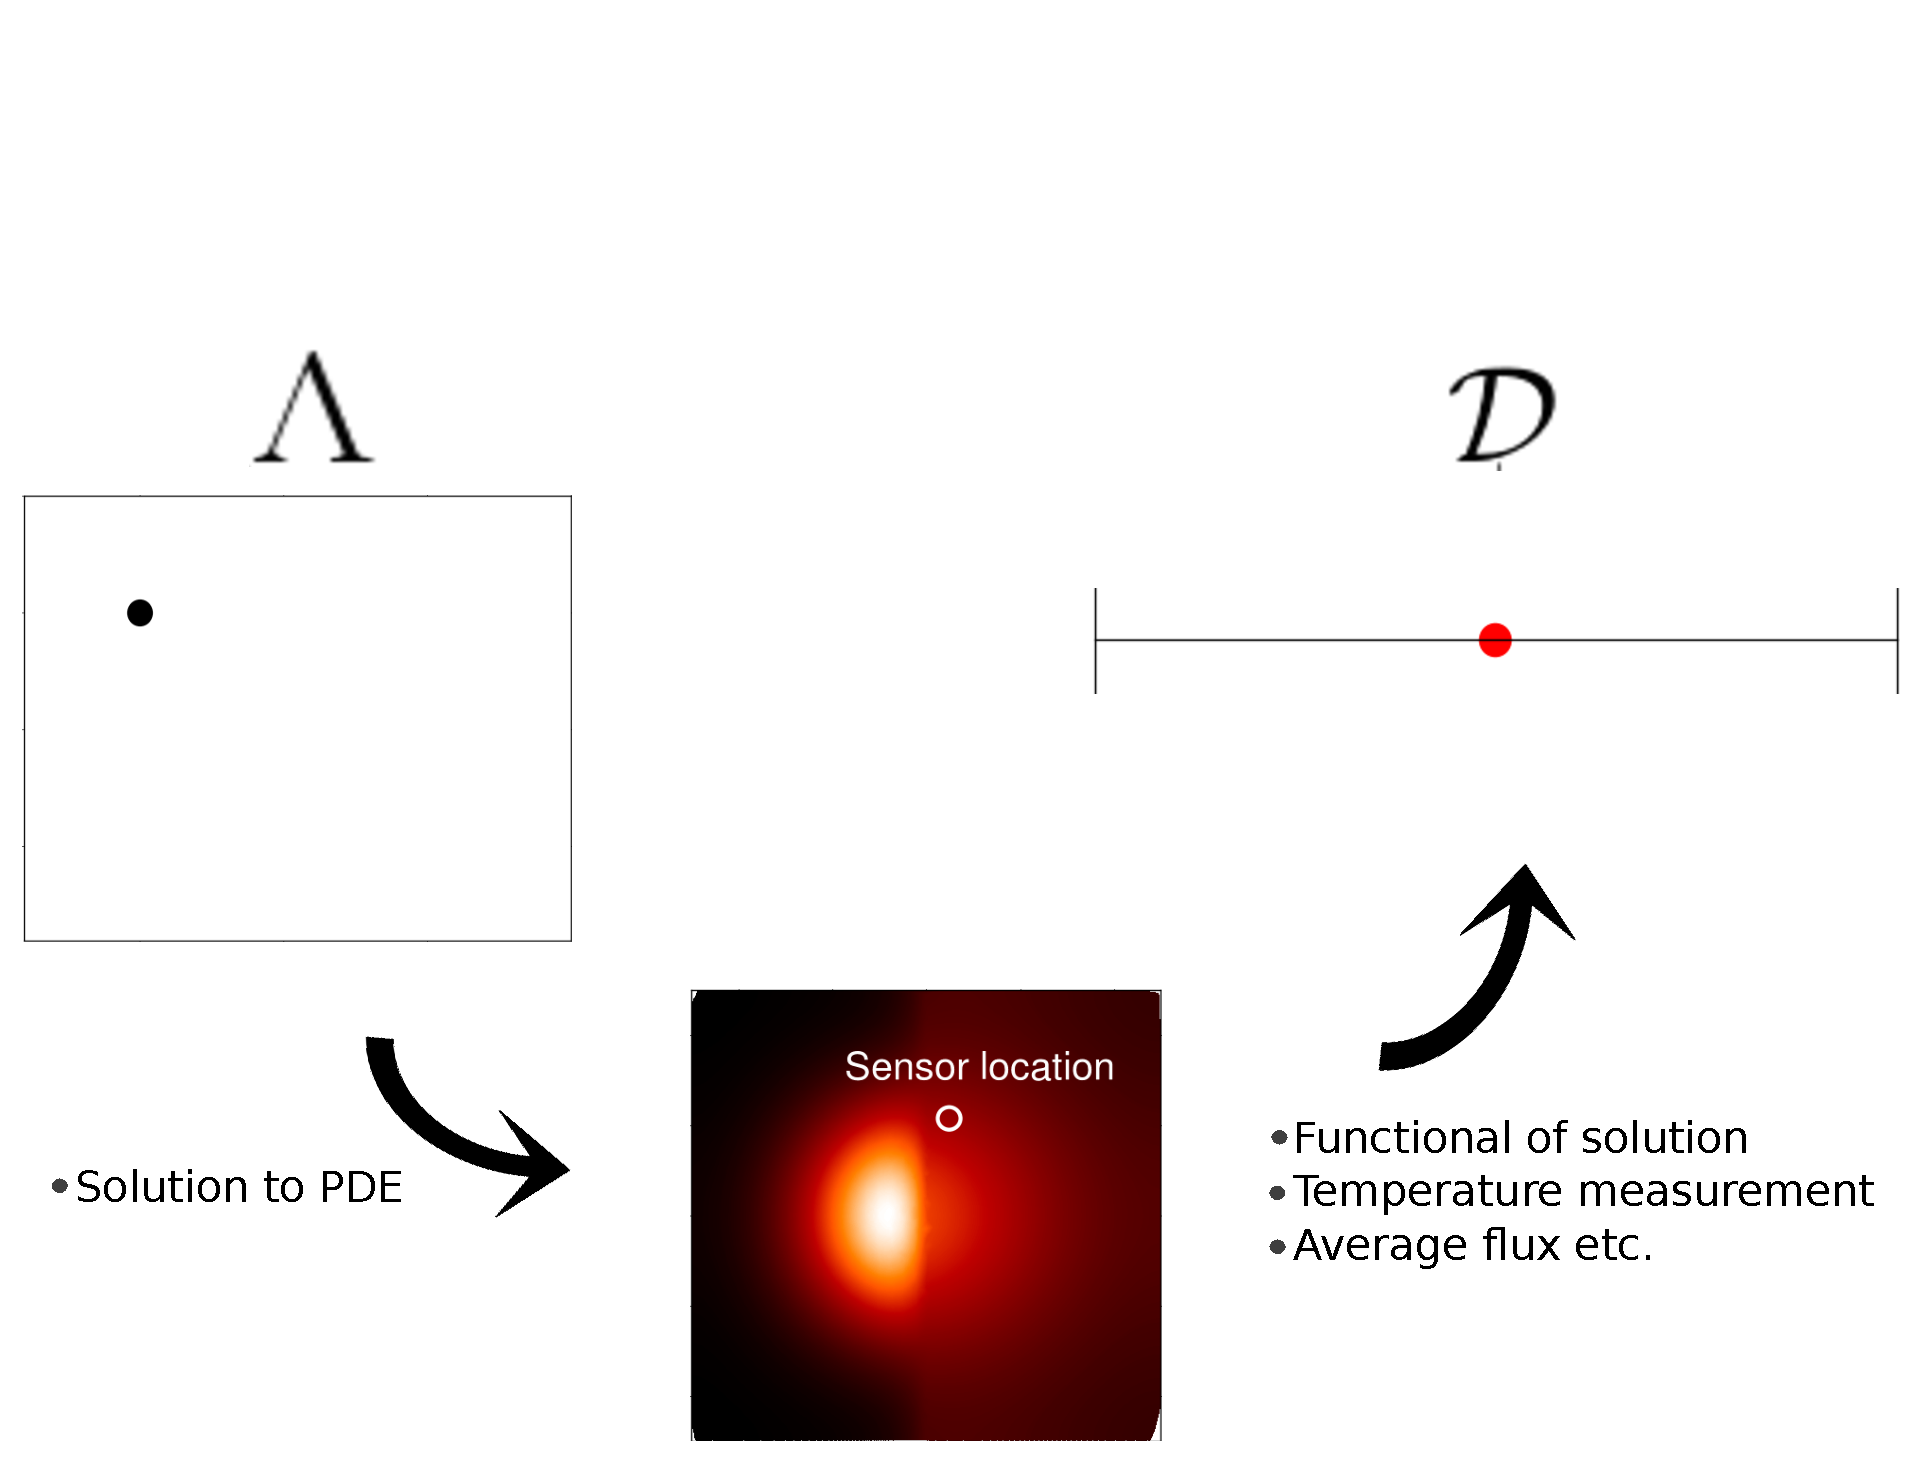
\includegraphics[width=0.85\textwidth]{./figures/threelevels/schematic_lambda_solution_data.pdf}
\end{figure}

}

\only<2>{

\begin{figure}[h]
	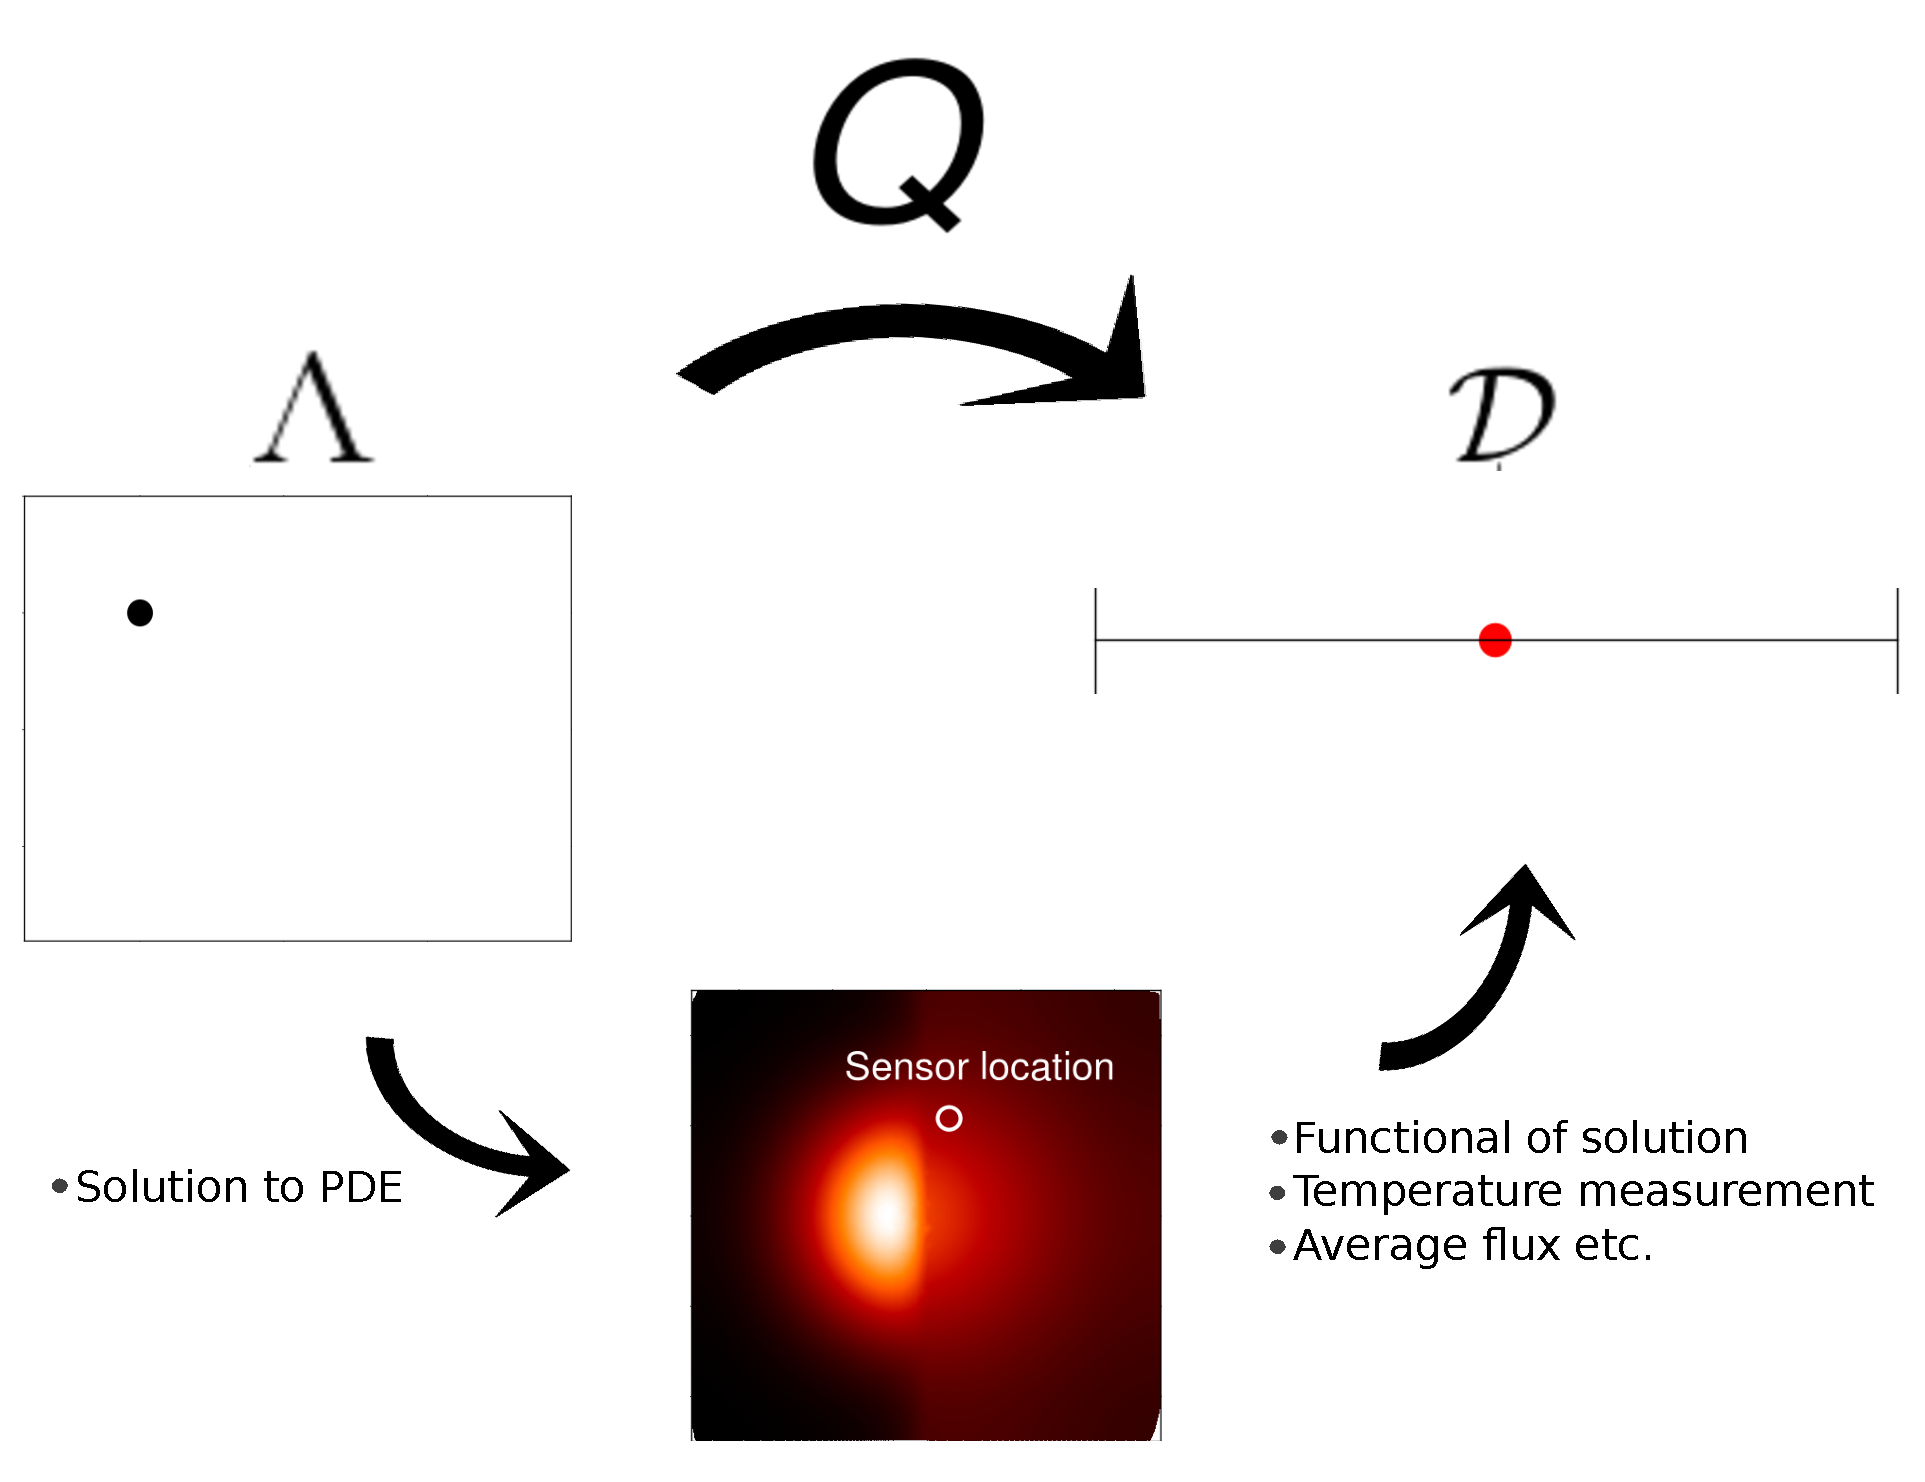
\includegraphics[width=0.85\textwidth]{./figures/threelevels/schematic_lambda_data.pdf}
\end{figure}

}

\only<3>{

\begin{figure}[h]
	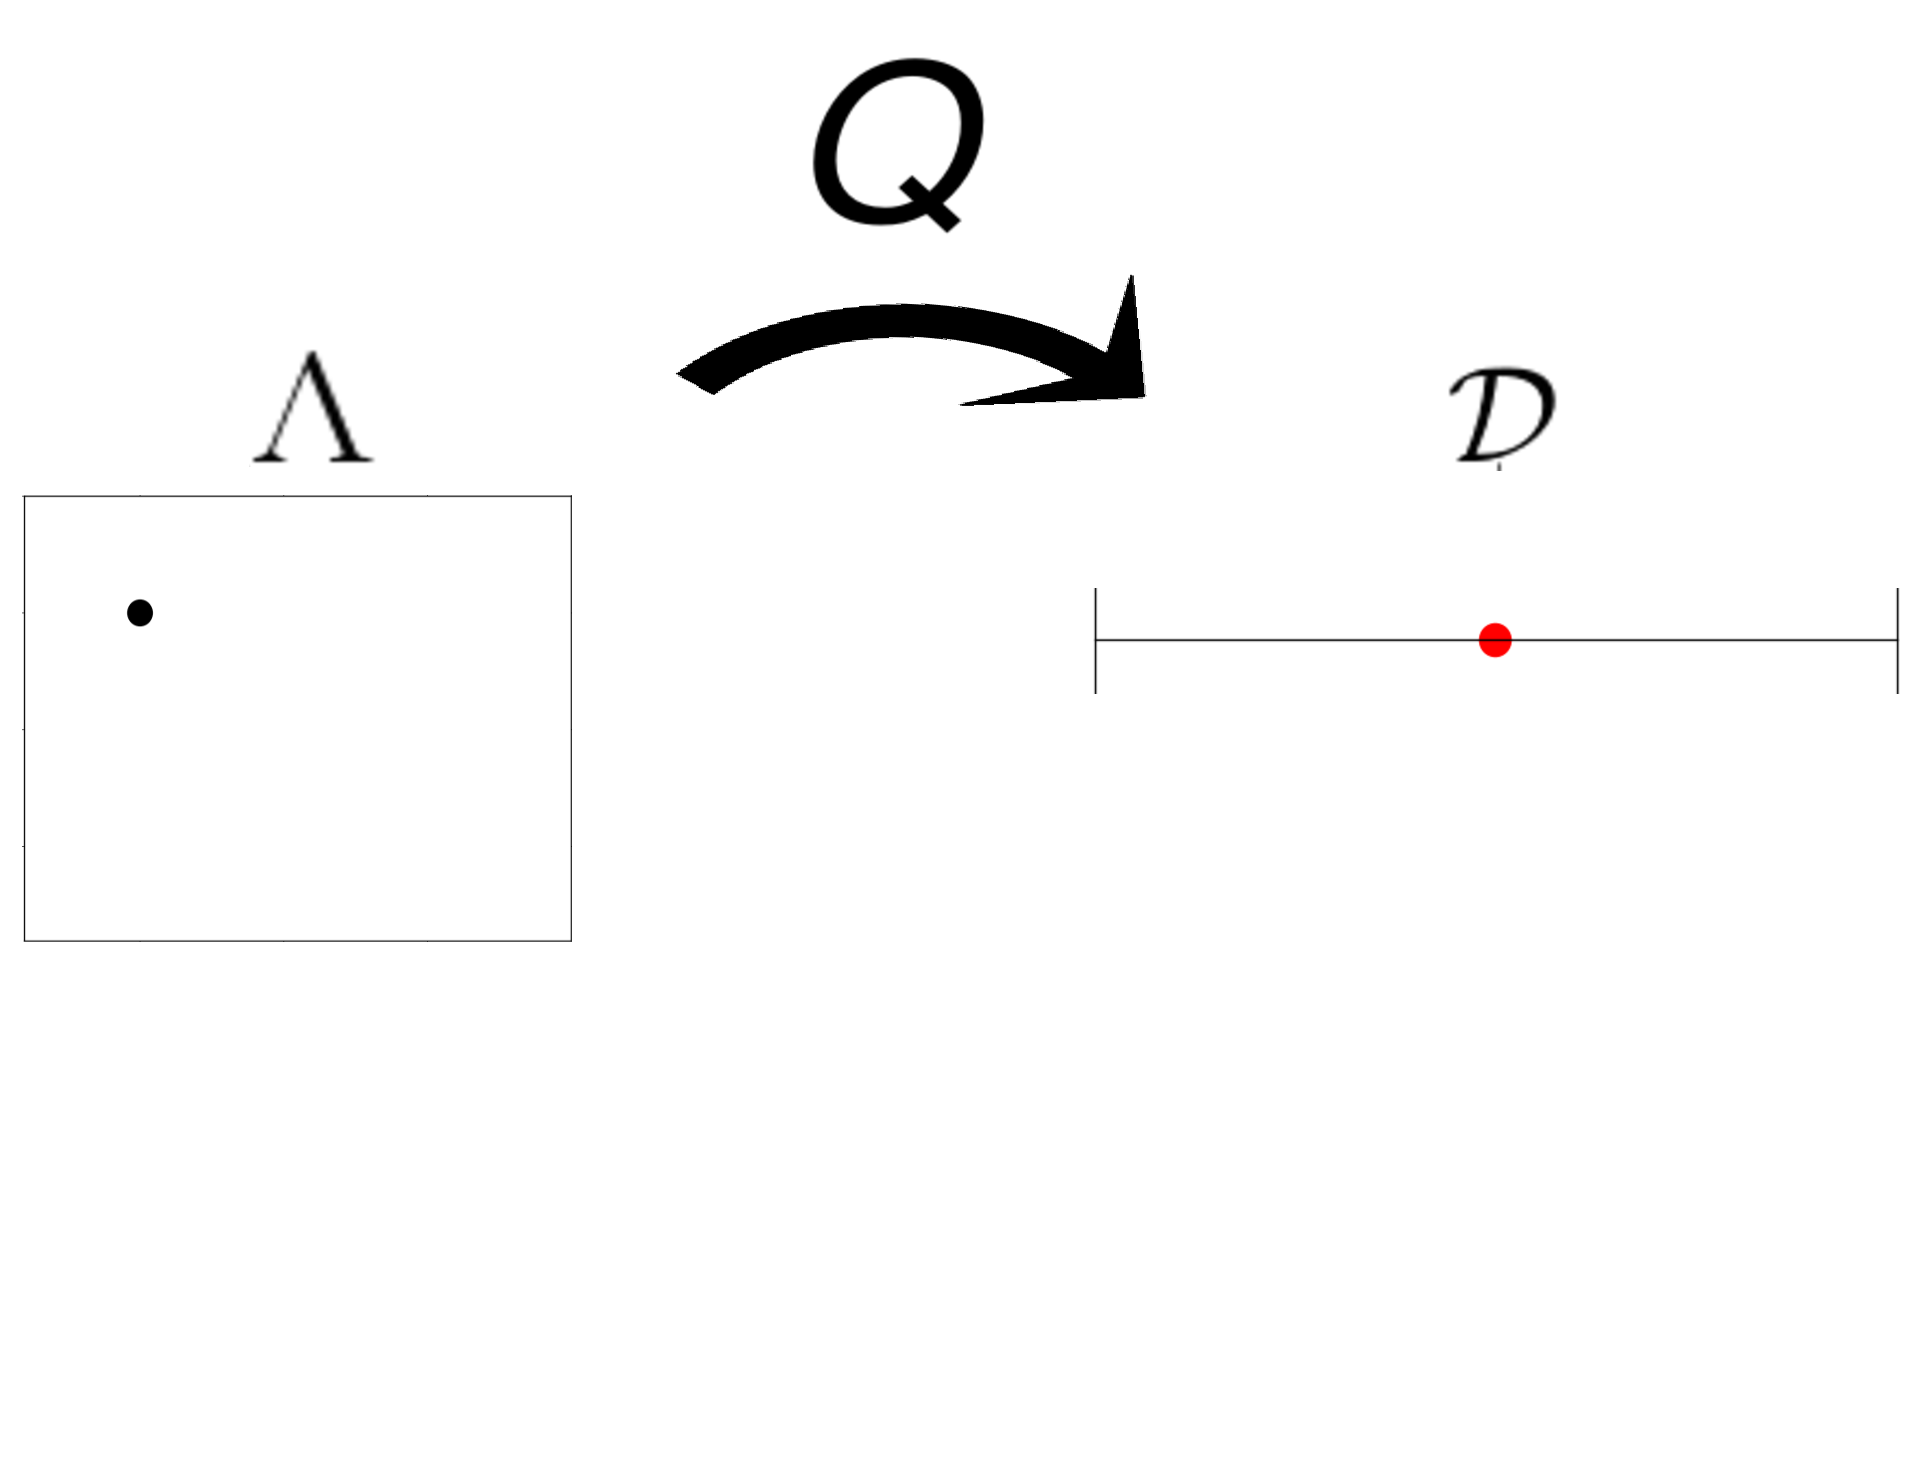
\includegraphics[width=0.85\textwidth]{./figures/threelevels/schematic_lambda_data_level1.pdf}
\end{figure}

}

\end{frame}

%%%%%%%%%%%%%%%%%%%%%%%%%%%%%%%%%%%%%%%%%%%%%%%%%%%%%%%%%%
\begin{frame}{A Forward UQ Problem}

\begin{figure}[h]
	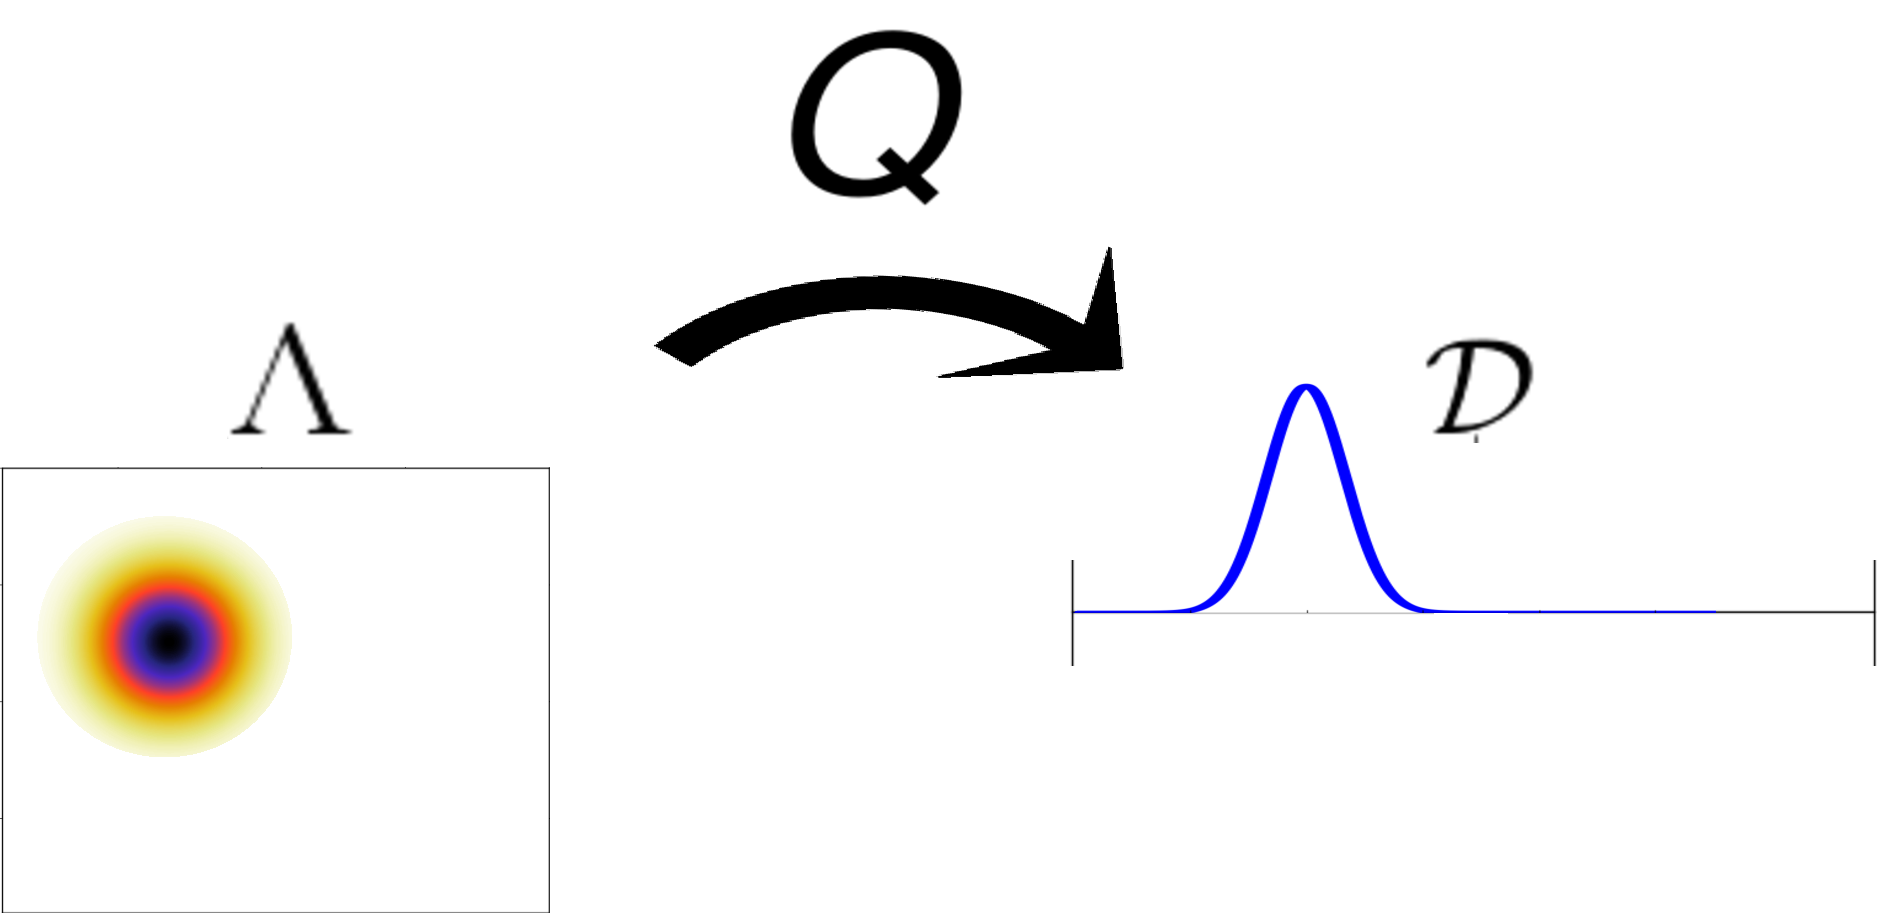
\includegraphics[width=0.85\textwidth]{./figures/threelevels/schematic_lambda_data_level3.pdf}
\end{figure}

{We denote the measurable spaces of parameters and data on the QoI as $(\pspace,\pborel)$ and $(\dspace,\dborel)$, respectively.}
\bigskip

\tdeepred{Given some prior density $\initial$ on $(\pspace,\pborel)$, we let $\predicted$ denote the push-forward of this density on $(\dspace,\dborel)$.}

\end{frame}

%%%%%%%%%%%%%%%%%%%%%%%%%%%%%%%%%%%%%%%%%%%%%%%%%%%%%%%%%%
\begin{frame}{The Inverse QoI Map}

\begin{figure}[h]
	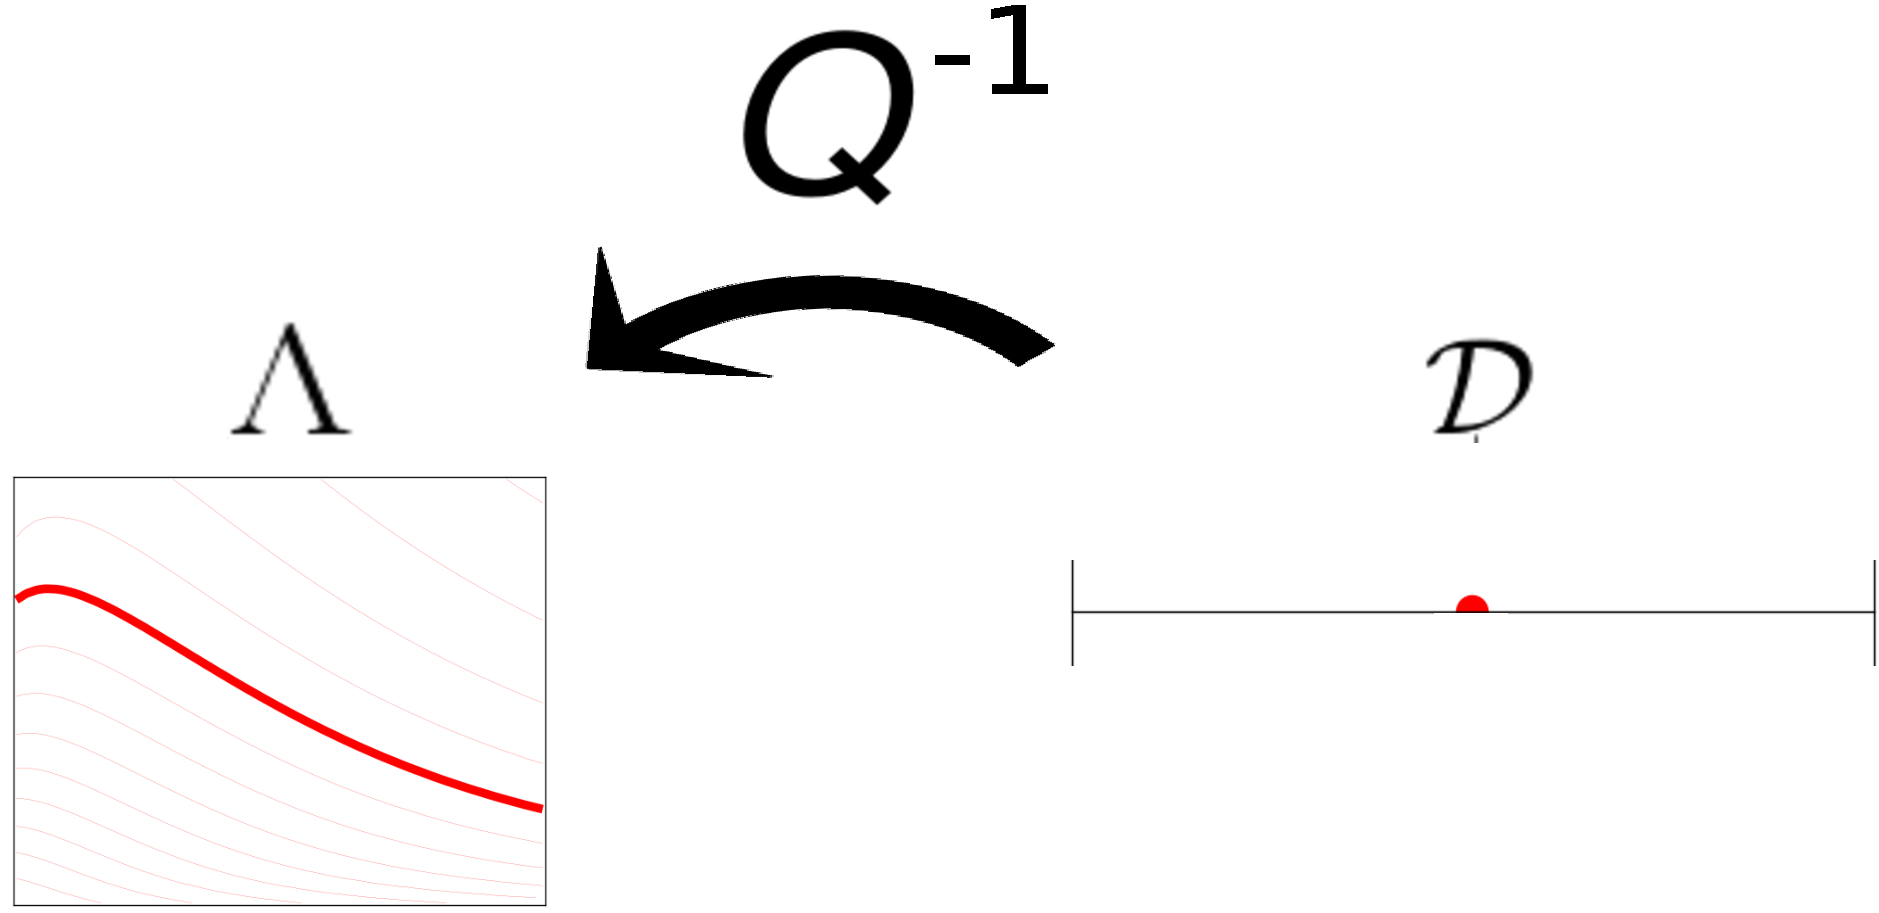
\includegraphics[width=0.85\textwidth]{./figures/threelevels/schematic_data_lambda_level1.pdf}
\end{figure}

\end{frame}

%%%%%%%%%%%%%%%%%%%%%%%%%%%%%%%%%%%%%%%%%%%%%%%%%%%%%%%%%%
\begin{frame}{An Inverse UQ Problem}

\begin{figure}[h]
	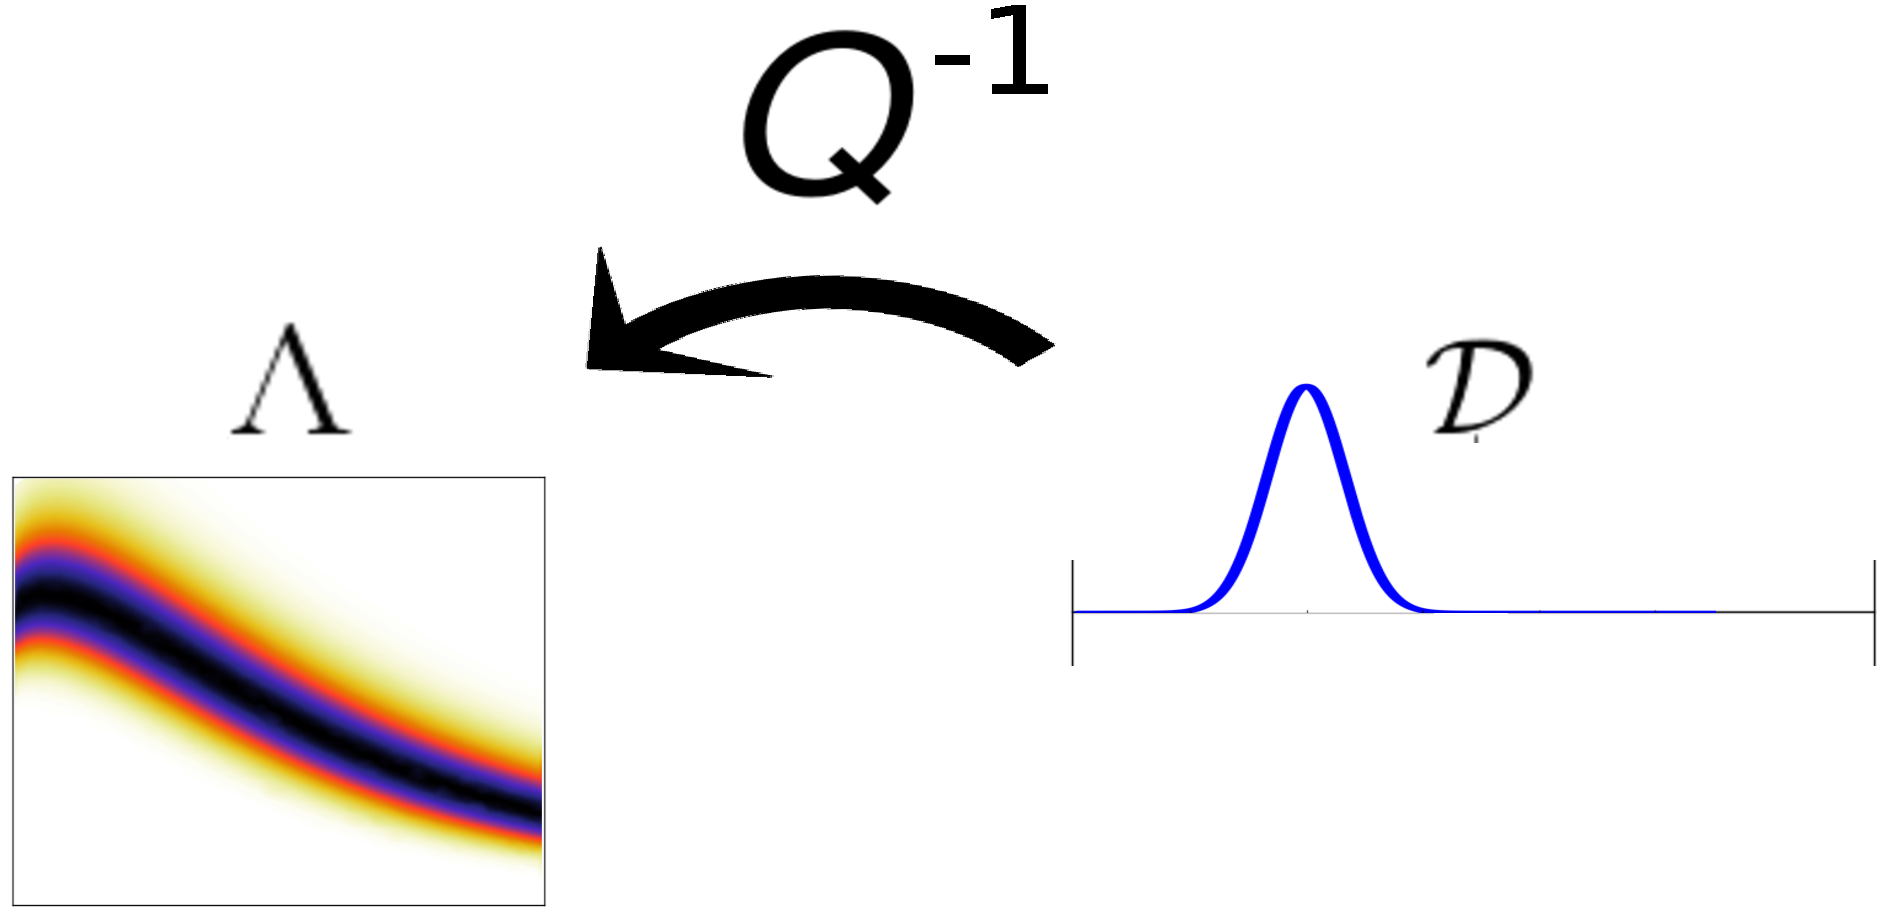
\includegraphics[width=0.85\textwidth]{./figures/threelevels/schematic_data_lambda_level3.pdf}
\end{figure}

\tdeepred{Given $\obs$ on $(\dspace,\dborel)$, we let $\predicted$ denote the pullback (consistent) density on $(\pspace,\pborel)$.}

\end{frame}


\subsection{Basic Assumptions \& Terminology}
%%%%%%%%%%%%%%%%%%%%%%%%%%%%%%%%%%%%%%%%%%%%%%%%%%%%%%%%%%
\begin{frame}[t]

\begin{itemize}[<+->]
	\item State variable: $u$ {\color{gray}(e.g. heat, energy, pressure, deflection)}
	\vskip 10pt
	\item<.-> Parameters: $\lambda$ {\color{gray}(e.g. source term, diffusion, boundary data)}
	\vskip 10pt
		\item Deterministic model: $\mathcal{M} (u, \lambda) = 0$, $$\mathcal{M}:\lambda \to u(\lambda)$$

	\item Quantity of Interest map \tdeepred{(QoI)} - at least pcw differentiable \vskip 5pt
		\begin{itemize}[<+->]
		\item Functional of the solution $$q: u(\lambda) \to \RR$$
		\item Can be vector valued $$Q = \mat{c}{q_1\\ q_2\\ \vdots \\ q_d}$$
		\item<.-> $Q(\lambda) := Q(u(\lambda))$
	\end{itemize}
	
\end{itemize}

\end{frame}


\subsection{The Stochastic Inverse Problem}
%%%%%%%%%%%%%%%%%%%%%%%%%%%%%%%%%%%%%%%%%%%%%%%%%%%%%%%%%%
\begin{frame}[t]

\begin{figure}
\centering
	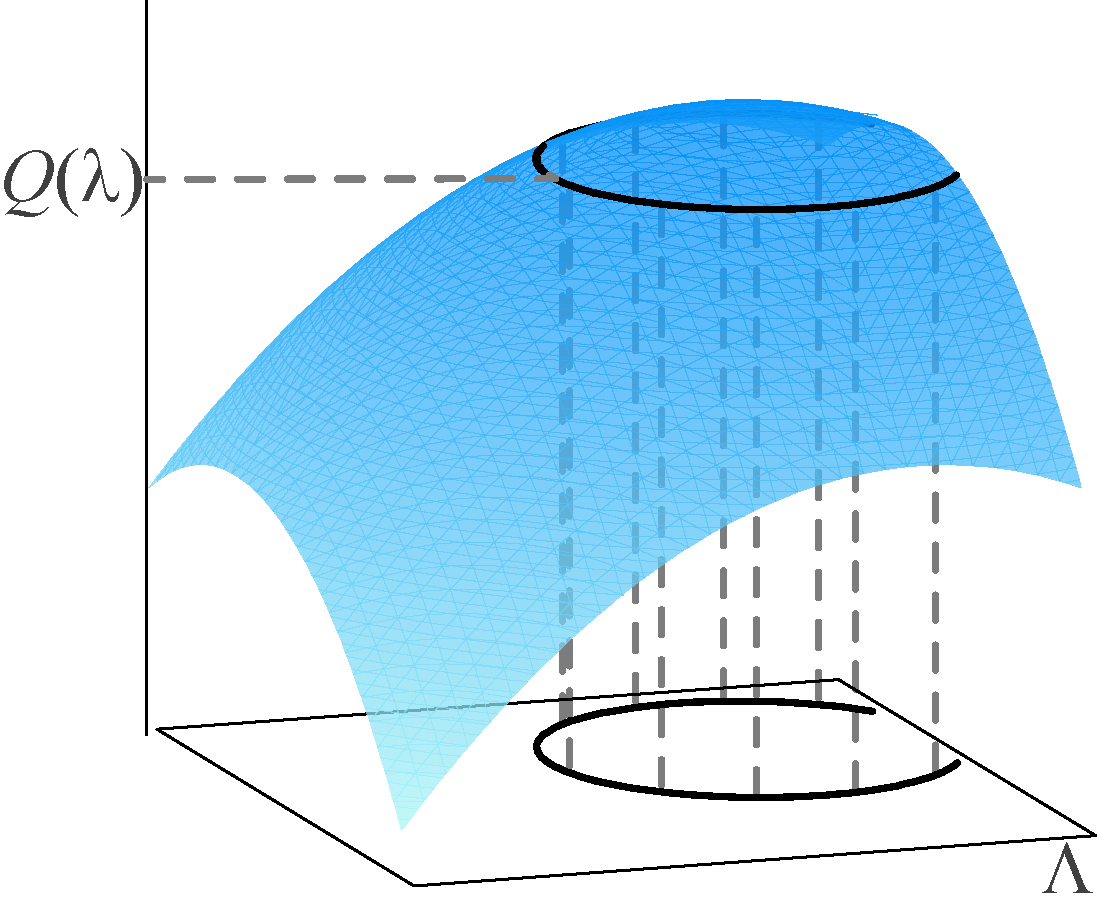
\includegraphics[width=.65\textwidth]{images/illustration1.pdf}<1>
	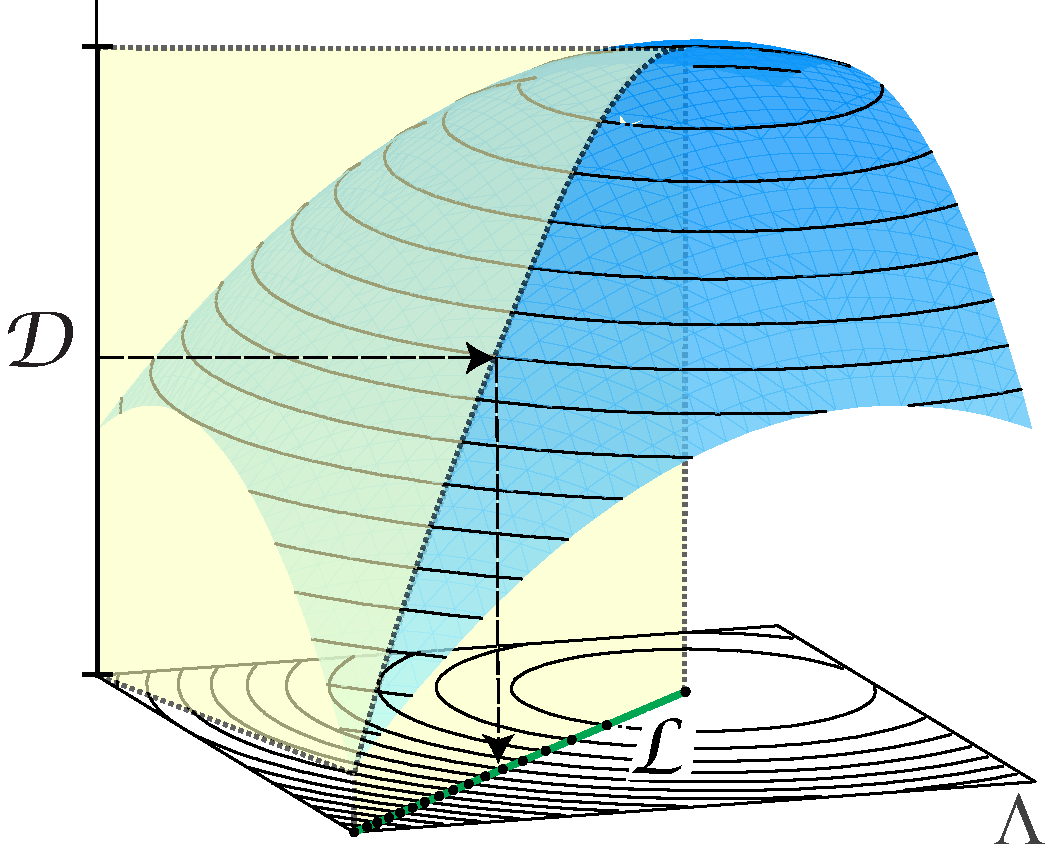
\includegraphics[width=.65\textwidth]{images/illustration2.pdf}<2>
	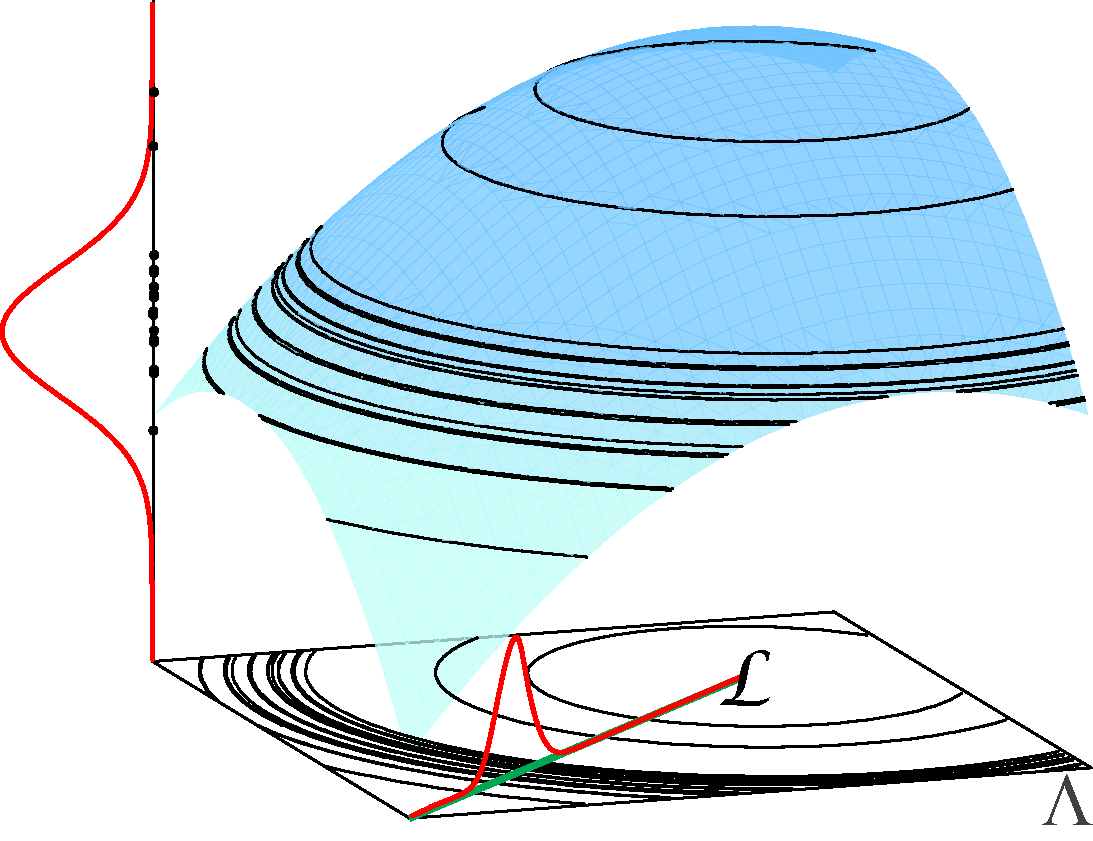
\includegraphics[width=.7\textwidth]{images/illustration3.pdf}<3>
\end{figure}
\begin{center}
{\scriptsize Figure adopted from \cite{BET14+} and used with permission}
\end{center}
\end{frame}

%%%%%%%%%%%%%%%%%%%%%%%%%%%%%%%%%%%%%%%%%%%%%%%%%%%%%%%%%%
\begin{frame}[t]

\begin{figure}
\centering
	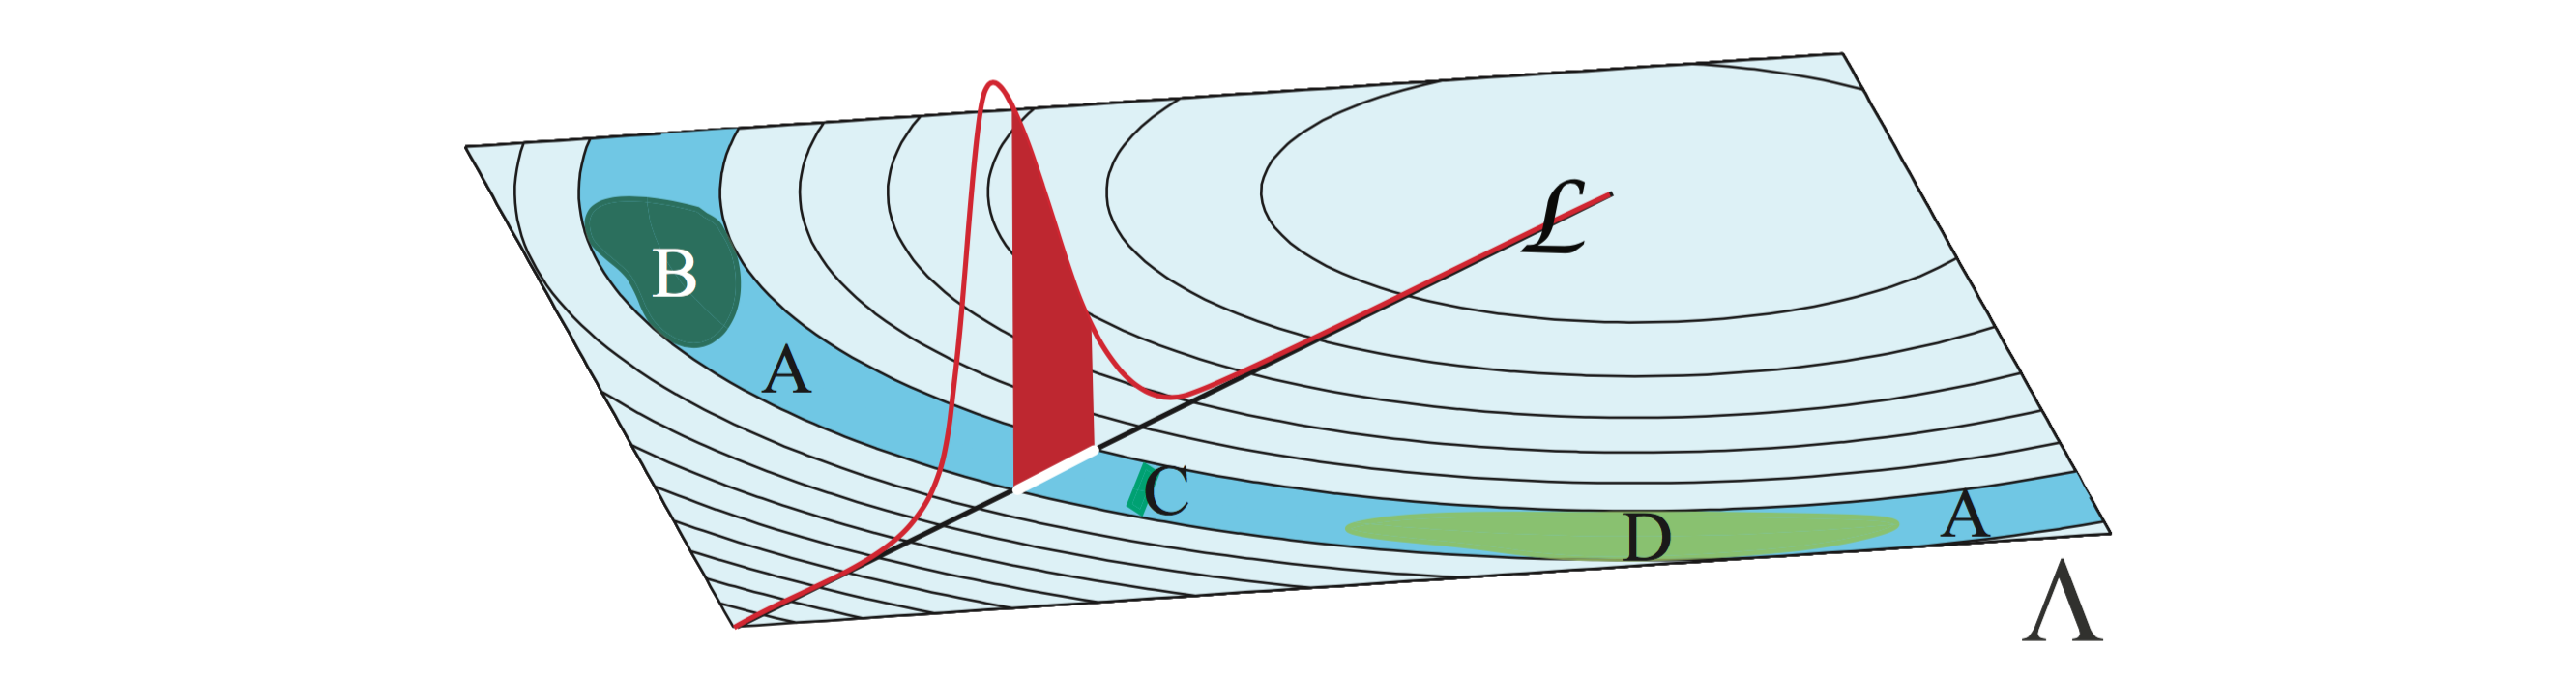
\includegraphics[width=1\textwidth]{images/troy_mt3contour.png}
\end{figure}
\begin{center}

{\scriptsize Figure adopted from \cite{BET14+} and used with permission}

\tdeepred{Key Question:} Distinguish (assign probability to) events that belong to same contour. 
\end{center}
\end{frame}
